% Complete journal draft, city-square exposure at 15 GHz.
% Build: pdflatex paper && pdflatex paper
\documentclass[journal]{IEEEtran}

\usepackage[T1]{fontenc}
\usepackage{amsmath,amssymb}
\usepackage{graphicx}
\usepackage{booktabs}
\usepackage{algorithm}
\usepackage{algpseudocode}
\usepackage[hidelinks]{hyperref}
\usepackage{cleveref}

% IEEE abbreviates figure and table references in running text.
\crefname{figure}{Fig.}{Figs.}
\Crefname{figure}{Fig.}{Figs.}
\crefname{table}{Table}{Tables}
\crefname{algorithm}{Algorithm}{Algorithms}

\graphicspath{{../FIGURES/}}

\newcommand{\uloc}{\hat{u}}
\newcommand{\uext}{\hat{v}}
\newcommand{\nhat}{\hat{n}}
\newcommand{\khat}{\hat{k}}
\newcommand{\x}{\mathbf{x}}
\newcommand{\dOmega}{\,\mathrm{d}\Omega}
\newcommand{\todo}[1]{\textbf{TODO: #1}}

\begin{document}

\title{City-square geometry sets relative pedestrian exposure at 15\,GHz}
\author{Robin~Wydaeghe%
\thanks{The author is with the Department of Information Technology, Ghent
University / imec, 9052 Ghent, Belgium.}}

\maketitle

\begin{abstract}
An absolute radio-frequency exposure level in a city square depends on base
station powers, positions, and counts that are neither public nor properties of
the square. This paper instead measures the exposure ratio, defined as the power
density at a pedestrian's head in the square divided by the power density that
the same network would give at the same point over open ground. Reciprocity
places the computation at the pedestrian. One outward ray trace then represents
every possible source position, and a photograph taken there sees the surfaces
that receive the early interactions. The photographs therefore measure the
material family that sets the bounce budget. The method was applied at 15\,GHz
to 880 standpoints in eleven photogrammetric city squares. The between-square
spread was 3.71\,dB for isotropic illumination, 4.93\,dB for rooftop sites, and
9.58\,dB for street cells. The largest within-square spread was 6.46\,dB, which
exceeded the isotropic between-square spread by 2.75\,dB. Image-based
discrimination among masonry materials moved the three distribution medians by
only 0.024, 0.029, and 0.022\,dB. This null bounds the claim to masonry squares
instead of weakening it. Full digital maximum ratio transmission cancels from
the ratio exactly, whereas geometric steering gives a one-sided upper bound.
At two people per square metre, bystanders reduced the street and rooftop ratios
by 1.4 and 1.0\,dB. A geometry-specific diffraction bound added median uplifts
of 0.06, 0.15, and 0.44\,dB. The ratio therefore isolates a repeatable property
of the square while retaining explicit error signs for the omitted physics.
\end{abstract}

\begin{IEEEkeywords}
15 GHz, adjoint ray tracing, electromagnetic exposure, photogrammetry,
radio-frequency propagation, urban geometry
\end{IEEEkeywords}

\section{Introduction}
\label{sec:introduction}

Radio exposure in a city is usually computed from a known deployment. A ray
tracer receives a list of base stations, solves one transmitter-receiver problem
for each link, and adds the fields or powers. This construction is appropriate
when the deployment is known. It cannot separate the effect of the square from
the effect of the operator's confidential site count, power, and placement.
Those network variables put the open-ground power density over nearly three
orders of magnitude, from 0.0075 to 3.0\,W/m$^2$ for rooftop sites and from
0.010 to 4.1\,W/m$^2$ for street cells. The general-public reference level at
15\,GHz is 10\,W/m$^2$~\cite{icnirp}. An absolute level therefore answers a
network question before it answers a city question.

The exposure ratio removes the unknown level. Its numerator is the power density
at the pedestrian's head in the real square. Its denominator is the power density
that the same network would give at the same point over open ground. Site power,
site density, and the absolute level divide out. The remaining number is one in
free space, less than one when buildings block more power than they return, and
greater than one when reflection wins. The ratio asks how the square changes
exposure, which is the quantity that can be compared between cities.

The location of the computation changes what can be measured. Conventional
tracing starts at each transmitter. The present trace starts at the pedestrian,
follows rays outward, and weights each escaped ray by the probability that a
site lies in its exit direction. Reciprocity then reads every path backward.
The familiar benefit is computational, since one trace replaces a trace for
each possible source position. The larger benefit is evidential. A street-level
photograph taken at the same point sees the surfaces that the early ray
interactions reach. Material family can then be observed instead of assigned,
and the distance over which the photographs retain that coverage sets the
bounce budget.

Existing city-scale exposure studies solve careful per-pair problems over known
base-station positions~\cite{leeman}. Earlier work by the same author also joins
photogrammetric geometry, propagation, and anatomical dosimetry for specified
deployments~\cite{wydaeghe2026}. The question here is different. No site list is
available, and the output must remain useful when a deployment model changes.
The point-centered ratio is therefore a physical separation between the
environment and the network, rather than a faster implementation of the same
per-pair calculation.

This paper makes four contributions. First, it applies a reciprocal outward
estimator to a continuous site distribution and preserves the arriving angular
power at the pedestrian. Second, it measures how much of each early interaction
lands on geometry visible from the same viewpoint, which reports for the first
time how co-located image evidence constrains an RF-exposure bounce budget.
Third, it compares the resulting ratio at 880 standpoints in eleven squares
under three illumination laws after measuring the crop radius. Fourth, it tests
the claim against material discrimination, matched and steered beams,
bystanders, truncation, polarization, and diffraction. The combination isolates
city geometry from deployment for RF exposure for the first time.

The remainder of the paper is organized as follows. Section~\ref{sec:related}
positions the estimator against per-pair tracing, deployment integration, image
materials, and adjoint transport. Sections~\ref{sec:ratio}--\ref{sec:valid}
define and check the method. Section~\ref{sec:results} reports the six result
beats. Section~\ref{sec:discussion} interprets them and states every known bias
with its sign. Section~\ref{sec:conclusion} concludes the paper.

\section{Related work}
\label{sec:related}

Deterministic radio ray tracers solve paths between named endpoints. Sionna RT,
for example, computes propagation paths between transmitter and receiver
antennas~\cite{sionna}. Leeman \emph{et al.} use that per-pair construction for
city-scale downlink exposure with base-station positions taken from public
conformity records~\cite{leeman}. The approach is physically detailed and
auditable. It gives path delay, phase, and diffraction for the deployment that
was supplied. Its cost and its output remain tied to that deployment, so a new
site layout requires a new set of link calculations. The present work replaces
that discrete input with a continuous angular distribution because no
deployment is known.

Stochastic deployment models already connect spatial site distributions to
exposure. Wiame \emph{et al.} compare stochastic geometry and deterministic ray
tracing in a Manhattan environment~\cite{wiame}. The LEXNET exposure index
precomputes normalized body coefficients and combines them later with a
deployment-dependent incident level~\cite{varsier}. These are close precedents,
not omissions in earlier work. The distinction here is that the environment and
the deployment remain separate before the body calculation. The square gives
an angular response, the possible sites give an angular illumination, and the
body receives their product. A scalar environment-and-deployment term cannot be
reweighted after it has discarded that angle.

Comparisons between cities are also established. Veludo \emph{et al.} measured
radio-frequency fields across microenvironments in ten European countries
\cite{veludo}. The earlier photogrammetric study by Wydaeghe \emph{et al.}
computed absorbed power density for specified outdoor deployments in more than
one city~\cite{wydaeghe2026}. The present contribution is therefore not the act
of comparing cities. It compares the property left after the same network is
divided out, and it does so at a frequency and angular resolution for which the
unknown deployment would otherwise dominate the result.

Image-derived radio materials are published as well. The mmSV pipeline segments
street-view images into material classes, projects them onto city geometry, and
uses them in millimetre-wave ray tracing~\cite{mmsv}. The present paper does not
claim that projection as new. Here the camera and the ray source share a
viewpoint. Co-location turns image coverage into a statement about which
surfaces the early interactions hit. The image is therefore used to bound what
the propagation model knows, rather than only to populate a material table.

Adjoint transport predates radio ray tracing. Veach gives the sensor-side
importance formulation used in rendering~\cite{veach}. Daylight coefficients
precompute a response to a discretized sky~\cite{tregenza}, and precomputed
radiance transfer stores a point response that can be combined with changing
illumination~\cite{sloan}. These works establish reciprocity, sensor-side
tracing, and source substitution. The contribution here is their use for a
deployment-averaged exposure ratio at a pedestrian, together with a measured
image-coverage budget and body coupling. The individual mathematical ingredients
are prior art.

\section{Exposure ratio}
\label{sec:ratio}

A person standing in a city square receives radio power from many base stations
at once. The buildings around them block part of that power and reflect part of
it back, so the total depends on the shape of the square as much as on any
single antenna. This paper computes that dependence as one number,
\begin{equation}
  \chi = \frac{S}{S_0} ,
  \label{eq:chidef}
\end{equation}
where $S$ is the power density arriving at the head in the real square and $S_0$
is the power density the same network would deliver at the same point over open
ground. This ratio is called the exposure ratio.

The ratio is the useful quantity because the network is unknown. An absolute
exposure in W/m$^2$ needs the transmit power, the number of sites and their
positions, none of which is public at millimetre wave frequencies and none of
which is a property of the square. Dividing by the free space answer removes all
three. What is left is a pure number that is 1 when the square is empty, below 1
where the buildings shadow more than they reflect, and above 1 where they
reflect more than they shadow. It transfers between cities, which a power
density does not.

Computing $\chi$ directly would mean placing a transmitter at every position a
base station could occupy and tracing rays from each one to the person. That is
the expensive way round. Instead everything is computed at the one point where
the person stands. Rays are launched from that point, followed until they leave
the square, and weighted by how likely a base station is to sit in the direction
each one left. \Cref{fig:adjoint} shows the idea.

Putting the transmitter and the receiver at the same point is what makes the
rest of the method possible, because a street level photograph taken from that
same point sees the surfaces the early bounces will hit. The material of a
facade is therefore measured rather than assumed, and how far that measurement
reaches is what sets how many bounces are worth following.
Section~\ref{sec:budget} returns to this and fixes the bounce budget from it.

\begin{figure*}[!t]
  \centering
  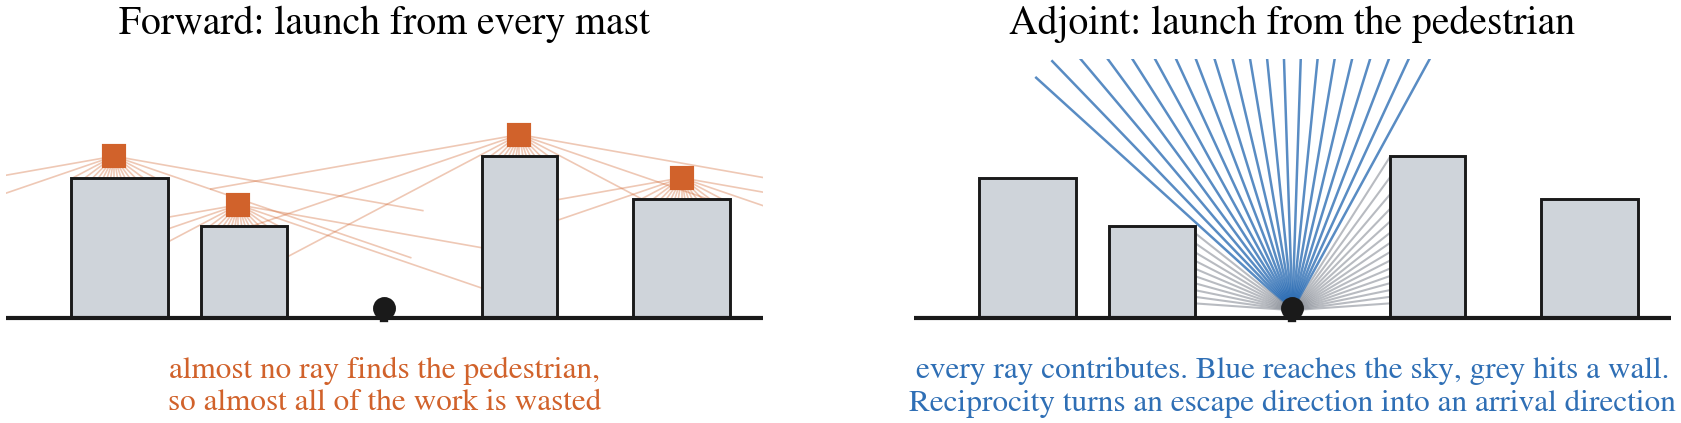
\includegraphics[width=\textwidth]{20_adjoint_idea}
  \caption{Rays are shot outward from the person rather than inward from the
  sources. A path is reversible, so a ray that leaves in direction $\uloc$ and
  escapes the square in direction $\uext$ carries the same attenuation as a ray
  arriving from a source in direction $\uext$ and reaching the person from
  direction $\uloc$.}
  \label{fig:adjoint}
\end{figure*}

\subsection{Notation}

Vectors are boldface, unit vectors carry a hat. $\uloc$ is a direction leaving
the observation point and $\uext$ is the direction in which a ray finally
escapes. Angles are measured from the horizon upward, so $\alpha$ is elevation
and $\alpha = 0$ is level with the head. \Cref{tab:symbols} lists the symbols
used in the equations.

\begin{table}[!t]
  \caption{Symbols}
  \label{tab:symbols}
  \centering
  \begin{tabular}{llc}
    \toprule
    Symbol & Meaning & Unit \\
    \midrule
    $\x$ & observation point, the head of the pedestrian & m \\
    $\uloc$ & direction leaving $\x$ & -- \\
    $\uext$ & direction in which a ray escapes the scene & -- \\
    $\alpha$ & elevation above the horizon & rad \\
    $r$ & horizontal range from $\x$ to a site & m \\
    $\rho$ & slant range from $\x$ to a site & m \\
    $h$ & height of a site above $\x$ & m \\
    $\nu$ & number of sites per unit volume & m$^{-3}$ \\
    $Q(\uext)$ & share of incident power per steradian of sky & sr$^{-1}$ \\
    $\Phi(\uloc)$ & power arriving per steradian, in units of $S_0$ & sr$^{-1}$ \\
    $S$, $S_0$ & arriving and free space power density & W/m$^2$ \\
    $\chi$ & exposure ratio, $1$ in free space & -- \\
    $w$ & power carried by one ray, $1$ at launch & -- \\
    $\Gamma$ & Fresnel reflection coefficient & -- \\
    $\theta_i$ & angle of incidence at a surface & rad \\
    $\kappa$ & fraction of reflected power that stays specular & -- \\
    $\sigma_h$ & root mean square surface roughness & m \\
    $\varepsilon_r$ & complex relative permittivity & -- \\
    $\lambda$ & wavelength & m \\
    $N$ & rays launched per standpoint & -- \\
    $M$ & cells in the launch grid & -- \\
    $L$ & largest number of surface interactions & -- \\
    $S_{\mathrm{inc}}$ & power density incident on a body facet & W/m$^2$ \\
    $S_{ab}$ & absorbed power density on the body & W/m$^2$ \\
    $T_0$ & power transmitted into tissue at normal incidence & -- \\
    $\nhat$ & outward normal of a body facet & -- \\
    $\khat$ & propagation direction of an incident wave & -- \\
    \bottomrule
  \end{tabular}
\end{table}

\subsection{Assumptions}

The method rests on seven assumptions, stated here because each one bounds what
the results can mean.

\begin{enumerate}
  \item[A1] \emph{Far field.} Every source is far enough away that it
  illuminates the square with a plane wave. The closest source position any
  model admits is 10\,m from the head, at the near edge of the street level
  band, and the array apertures involved are under 0.3\,m, whose far field
  begins at $2D^2/\lambda = 9$\,m at 15\,GHz. The margin is thin only for the
  very nearest street level sources and is wide everywhere else.
  \item[A2] \emph{Powers add, phases do not.} Contributions from different
  paths are summed in power. At 15\,GHz and a 100\,m range, the phase of a path
  turns by about $3.1 \times 10^{4}$\,rad per radian of change in the exit
  angle, so resolving it would need on the order of $10^{10}$ angular cells
  against the 512 used here. Any phase this method could carry would be noise.
  \item[A3] \emph{Sites are a density, not a list.} Base station positions are
  unknown and are modelled as a uniform density over a slab of ground, bounded
  in height and in range. Section~\ref{sec:illum} builds the model.
  \item[A4] \emph{Every site delivers the same power at the head.} Sites are
  counted rather than weighted by their range, so the angular distribution of
  incident power follows the angular distribution of site count. The reason is
  that each site is built to serve its own cell and sets its power to cover it,
  so a nearer site is not a proportionally louder one. That is an assumption
  about how a network is operated rather than about how waves travel, and
  Section~\ref{sec:illum} carries the alternative through as a sensitivity. The
  choice is not cosmetic: the street level
  model places 88\,\% of its measure below $5^\circ$ under counting and 42\,\%
  under spreading, and elevation weighting is what separates one square from
  another.
  \item[A5] \emph{Surfaces are locally flat.} Each triangle is treated as a
  smooth interface with a Gaussian height error of standard deviation
  $\sigma_h$ about its own plane.
  \item[A6] \emph{No diffraction.} Energy bending around building edges is
  absent. The three paragraphs after this list give the reason and the
  direction of the resulting error.
  \item[A7] \emph{Unpolarised.} Reflection uses the average of the two
  principal polarisations rather than tracking a polarisation state.
\end{enumerate}

A6 is the assumption a reader is most likely to challenge, so it gets the space
here. Four things make it defensible at this frequency and for this quantity, and
the last of them is a bound computed on the same geometry rather than an argument
carried over from someone else's.

The first is that it has been measured, at almost this frequency and in this
kind of geometry. A street microcell campaign at 2.44, 14.8 and 58.68\,GHz, with
matched antennas and bandwidth equalised across the three bands, found the
excess loss behind a building corner growing at 3.0 to 3.5\,dB per decade of
frequency, against the 10\,dB per decade of the corner diffraction model drawn
on the same axes \cite{ericsson, mmmagic}. At one location in that campaign, at
58.68\,GHz, a manual trace of the power delay profile found no arrival above the
noise floor at the delay the path around the corner would have occupied. What
arrived first there was attributed instead to scattering from rough surfaces
near the corner, and the strongest arrival, 20\,dB above the rest of the
profile, matched a path of four specular reflections off exterior walls. That
last peak was not seen at most of the other shadowed locations, so the campaign
carries the weaker claim rather than the stronger one: what reaches a shadowed
receiver in a street is not diffracted power, whether it arrives specularly or
by scattering. The mechanism is the ordinary one: a diffracted
field falls off relative to the field that produced it as $1/\sqrt{ks}$ with
distance $s$ from the edge, which at 15\,GHz and 10\,m is about $1/56$ in
amplitude, near 35\,dB down in power. Diffraction is a correction to a picture
that reflection already describes, which is the opposite of its role at the
metre wavelengths where street models were first built and where an edge is only
a few wavelengths away from everything.

The second is where that correction would actually lead, and it applies to one of
the two bands and not to both. Diffraction dominates only in deep shadow, at
points no direct or reflected path reaches, and the standpoints used here are
required to have open sky above them, with points that have no sky discarded
before any trace runs. For the street cell band that closes the question, because
those sites sit from 2.5 to 6.5\,m above the head, below the roofline, and every
direction the model blocks is blocked by a facade. For the rooftop band it does
not. Those sites sit 13.5 to 43.5\,m above the head, above a typical European
roofline, and open sky above a standpoint is the precondition for a path over a
roof rather than a defence against one. Measurements in Manhattan street canyons
with a rooftop site some 20\,m above the surrounding buildings found the over the
top mechanism beating street level scattering by 7\,dB in fit error
\cite{adhikari}. For the rooftop band the argument therefore rests on the next
two items and not on this one.

The third is that the error has a known sign. A diffracted path can only deliver
power the trace does not currently collect, never remove any, so leaving it out
biases $\chi$ low. That holds because A2 adds powers rather than fields. Were the
estimator coherent, a diffracted contribution could arrive out of phase and the
sign argument would fail. Every value reported here is a lower bound with respect
to this term, and the shortfall grows with how narrow and how enclosed the street
is. That is the right direction for an omission to run in an exposure study, and
it is stated rather than assumed away.

The fourth is the size of it, measured here. A dense mask of 720 azimuths by 600
elevation bands is cast at each standpoint on the same meshes and the same
standpoint coordinates as the reported runs. Every shadowed direction is given a
Fresnel-Kirchhoff parameter $\nu = \theta\sqrt{2d/\lambda}$ and its knife edge
loss \cite{p526} is integrated against the same illumination measure the
estimator uses. The
mask first has to earn trust, and it does: integrated over the \emph{visible}
directions instead, it reproduces the tracer's own direct term to within 0.34\,\%
for the isotropic model, 1.73\,\% for rooftop and 7.3\,\% for street, by an
independent code path with an independent quadrature. Over the 20 most enclosed
standpoints of the 3 most enclosed squares, the resulting uplift on $\chi$ has a
median of 0.06\,dB isotropic, 0.15\,dB rooftop and 0.44\,dB street. Every choice
in that calculation errs upward, so it is a bound and not an estimate: a single
absorbing half plane, a distant source, no re-blocking, a knife edge rather than
a lossy wedge, and the diffracted term multiplied by each standpoint's own
multipath gain so that paths which diffract and then reflect are covered. Against
a spread of 8.1\,dB within a single square, 0.15\,dB changes nothing. Repeating
the same calculation at 2\,GHz raises those medians to 0.18, 0.53 and 1.82\,dB, a
factor of 3.1 to 5.0, which reproduces the frequency argument of the first item
on this geometry rather than borrowing it.

The street cell model is the exception and it is not a small one. That model puts
87.9\,\% of its measure below 5\textdegree{} of elevation, its worst standpoint
takes an uplift of 12.6\,dB, and at 4 of the 60 standpoints its entire elevation
support is occluded, so the direct term is exactly zero and every watt in the
answer has arrived by reflection. Those standpoints also carry the smallest
absolute $\chi$ in the study. For that model in that geometry the omitted term is
not a correction, and no argument here is offered that it is.

Two limits on the borrowed half of this. There is a body of work in which a
diffraction shaped model fits around a corner at 28\,GHz better than a scattering
one does, which read alone points the other way. It does not survive reading the
fitted constant: the corner loss that fits is about 2\,dB, against a theoretical
edge coefficient near 40\,dB down at that frequency \cite{duchizhik}. The
functional form wins and the mechanism it is named after is not what supplies the
power. And all of the published decompositions of shadowed power into diffracted
and reflected parts were measured in street canyons, which waveguide, rather than
in open squares. A square presents fewer facades per unit solid angle, so the
reflected budget that stands in for diffraction here is thinner than it is where
the substitution was measured. No open square decomposition exists at any
frequency to check that against. This is also where the largest untested weight
sits, since ablating diffuse scattering rather than diffraction is what moves
published prediction error the most at these frequencies \cite{vitucci}.

A7 needs a word too, because the usual defence of it is not available at this
frequency. That defence says the multiply reflected tail is depolarised, so
averaging the two polarisations is exact for it. Measured cross polarisation
ratios say otherwise: pooled over many campaigns a path with no excess loss sits
near 28\,dB, falling by about half a decibel for every decibel of excess loss
\cite{karttunen}. An even split would need some 56\,dB of excess loss, and a
path that far down carries nothing. The tail that matters is not depolarised.

What the average costs can be bounded instead, and the bound has two sides. A
vertical facade struck by a near horizontal ray presents a nearly horizontal
plane of incidence, so a vertically polarised network field meets it in the
transverse electric case, where the unpolarised mean is never wrong by more than
3.0\,dB and errs low. The transverse magnetic case has a deep minimum near
$66^\circ$ of incidence for concrete, where the mean can err high by tens of
decibels on one bounce. That geometry arises on the ground rather than on a
facade, and only for arrivals within a few degrees of $24^\circ$ elevation, a
band holding 7.8\,\% of the rooftop model's measure and 0.4\,\% of the street
model's. So the approximation is bounded and biased low on facades, and
unbounded but rare on the ground.

The remaining sections describe the scene, the illumination model, the ray
estimator, the body, and the checks that constrain them.

\section{Configuration}
\label{sec:config}

The scene is a photogrammetric mesh of a real square, cut to a cylinder of
radius 250\,m about the standpoint and reaching from the ground to the roofline.
The mesh comes from aerial and street level imagery and carries no material
information of its own, so classes and electromagnetic parameters are assigned
afterwards. Radius 250\,m is not a free choice and Section~\ref{sec:valid}
reports what sets it. It should not be confused with the 250\,m that appears
in \cref{tab:models} as the far edge of the rooftop range band. One says how
much geometry is kept around the standpoint, the other how far away a base
station is allowed to be. They are fixed by different arguments and happen to
agree.

\subsection{Surfaces and materials}
\label{sec:materials}

Every triangle is assigned one of a small set of classes. In the baseline run
the class follows from geometry alone, splitting near horizontal faces at ground
level from near vertical faces above it, with vegetation separated by its
surface roughness at the mesh scale. Each class carries a complex relative
permittivity from the ITU building materials recommendation \cite{itu2040} at
15\,GHz and a root mean square roughness $\sigma_h$ from published surface
metrology on the corresponding material.

An optional path replaces the geometric class with one read from street level
photographs. Panoramas are segmented, registered to the mesh by matching the
skyline they see against the skyline the mesh casts, and their labels are
projected onto the triangles each panorama can see. Two models are used and they
answer different questions. A semantic segmentation network trained on street
scenes names the object, which separates a building from a tree from a road
surface but has one class for every facade regardless of what it is made of. A
promptable segmentation model is then asked for the material within those facade
regions, which is the axis the first model cannot resolve \cite{sam}. The
registration and projection are described in the supplementary information.

Imagery comes from two providers and the split matters when reading coverage.
Squares represented by a single panorama use one provider's official captures,
while the multi-station route at the reference square comes from a second,
community sourced provider, which is the only set carrying the material axis.
The comparison between the geometric and the image derived assignment is a
result rather than part of the method, so it is reported separately. One thing
belongs here rather than there, though. The cross city comparison is run with
geometric classes at every square and carries no image evidence at all. The
photographs enter at the reference square, which is where the material path is
demonstrated and where the coverage figures of Section~\ref{sec:budget} are
measured. What limits the others is registration rather than imagery, and
until that is fixed the image derived arm can claim one square.

What the photographs buy is worth stating plainly, because it is easy to expect
the wrong thing of them. They are not a fine adjustment to the permittivity.
Reflection at 15\,GHz varies little across the materials ordinary European
squares are actually built from, so moving between brick, stone and rendered
masonry shifts $\chi$ by far less than any difference this paper reports. The
job the photographs do is to establish which family of materials the square
belongs to at all. A square faced in glass and metal would fall outside that
family, and there the geometric default would be wrong rather than
approximate, with nothing in the mesh itself to reveal it. So the image evidence
licenses the geometric assignment instead of competing with it, and it is also
what bounds the claim: the results below are stated for masonry squares because
masonry is what was observed. It is family membership, not permittivity, that
Section~\ref{sec:budget} uses to set the bounce budget.

\subsection{Standpoints}

Exposure is not evaluated at one point. Each square contributes 80 standpoints and
results are reported as a distribution over them rather than as a single value,
because the spread within one square is comparable to the spread between
squares, so a single point would hide most of the variation.

Where a person can stand is decided from the mesh and not from a map. A grid of
columns at 3\,m spacing is laid over the crop, a ray is dropped down each one,
and the column is kept when it lands on a near horizontal face at the square's
ground level with enough clearance that a head at that position is not inside a
wall or a stall. A second filter drops any candidate whose head sees less than
1\,\% of the sky, which removes positions buried under an arcade or inside a
passage. That filter matters again later, because it is why no standpoint sits
in the deep shadow where the diffraction term left out by A6 would be the
leading one. Kept columns are then chained by nearest neighbour, which fixes
an order for plotting and for the step statistics but has no effect on any
exposure value, since each standpoint is traced independently. No street
centreline, footway polygon or other map layer is used, so the sampling does not
inherit whatever a mapping provider decided a street is.

The grid keeps far more candidates than are traced, so the chain is subsampled
at even spacing along its length down to the 80 that are reported. Subsampling
the chain rather than taking its first 80 links keeps the reported set spread
over the whole square instead of piled up at whichever end the chain began.

This set of standpoints is distinct from the route the photographs were captured
along, and the two should not be confused. The capture route is wherever the
imagery provider drove or walked, and it determines what the panoramas see. The
standpoints are where exposure is evaluated. They overlap but are neither equal
nor derived from one another.

\section{Illumination model}
\label{sec:illum}

Where the base stations are is unknown, so the model integrates over where they
could be. Operators do not place millimetre wave sites at arbitrary heights and
ranges: a site sits either on a roof or on street furniture, and beyond some
range its contribution stops mattering. Those two facts bound the region a site
can occupy, and what this section builds from that region is the one function the
estimator needs, the share $Q(\uext)$ of the incident power that reaches the head
from each steradian of sky.

\subsection{Sites per steradian}

Take sites spread uniformly through a slab, with $\nu$ sites per unit volume, at
heights between $h_{\min}$ and $h_{\max}$ above the head and at horizontal
ranges between $r_{\min}$ and $r_{\max}$. Look outward from $\x$ in a direction
at elevation $\alpha$, along a narrow cone of solid angle $\dOmega$. The number
of sites in that cone is the number in the part of it that lies inside the slab
and inside the range band,
\begin{equation}
  \mathrm{d}N = \nu \dOmega \int_{\rho_-(\alpha)}^{\rho_+(\alpha)} \rho^2 \,
  \mathrm{d}\rho
  = \frac{\nu}{3} \left[ \rho_+^3(\alpha) - \rho_-^3(\alpha) \right] \dOmega .
  \label{eq:cone}
\end{equation}
A site at slant range $\rho$ and elevation $\alpha$ has height $\rho \sin\alpha$
and horizontal range $\rho \cos\alpha$, so each band clips the cone from one
side,
\begin{align}
  \rho_-(\alpha) &= \max\!\left( \frac{h_{\min}}{\sin\alpha},
  \frac{r_{\min}}{\cos\alpha} \right), \nonumber \\
  \rho_+(\alpha) &= \min\!\left( \frac{h_{\max}}{\sin\alpha},
  \frac{r_{\max}}{\cos\alpha} \right).
  \label{eq:caps}
\end{align}
\Cref{fig:elevation} draws the geometry behind \eqref{eq:cone}.

What the estimator needs is not a count of sites but a share of incident power.
Under A4 the two are the same function up to a constant, because every site
contributes equally, so
\begin{equation}
  Q(\uext) \;\propto\; \rho_+^3(\alpha) - \rho_-^3(\alpha)
  \label{eq:Q}
\end{equation}
wherever $\rho_+ > \rho_-$, and $Q = 0$ elsewhere. Only elevation appears,
because a uniform density of sites on level ground has nothing to distinguish one
compass bearing from another. Counting sites rather than weighting them by range
is what makes $r_{\max}$ load bearing: the $\rho^2$ inside \eqref{eq:cone} says
far sites are the numerous ones, so where the range band ends decides how much of
the answer they own. Weighting each site by its own free space spreading
$1/\rho^2$ instead replaces the cubed bracket in \eqref{eq:Q} with
$\rho_+ - \rho_-$, and that variant is carried through as a sensitivity.

\begin{figure*}[!t]
  \centering
  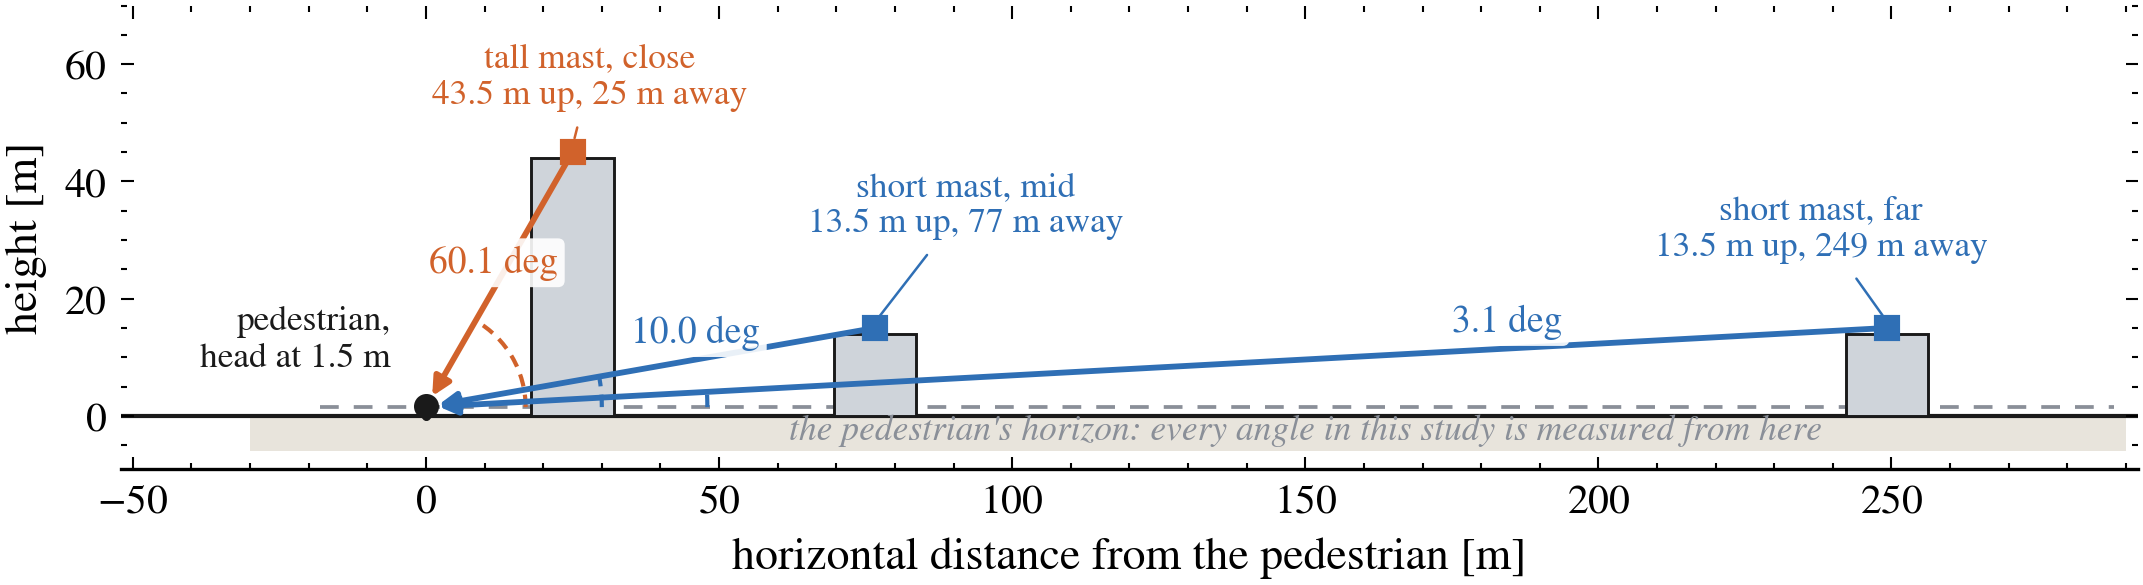
\includegraphics[width=\textwidth]{18_elevation_geometry}
  \caption{A site at horizontal range $r$ and height $h$ above the head is seen
  at elevation $\alpha$ with $\tan\alpha = h/r$. Near sites appear high in the
  sky and far sites appear near the horizon, so a band of heights and a band of
  ranges together fix which elevations can hold sites at all.}
  \label{fig:elevation}
\end{figure*}

Two consequences follow directly and both matter. First, the support is not a
free parameter. A direction can hold a site only when $\rho_-(\alpha) \le
\rho_+(\alpha)$, which gives
\begin{equation}
  \arctan \frac{h_{\min}}{r_{\max}} \;\le\; \alpha \;\le\;
  \arctan \frac{h_{\max}}{r_{\min}} ,
  \label{eq:support}
\end{equation}
so writing down a height band and a range band already fixes the elevation
limits. Second, the near horizon carries most of the measure, and the near
horizon is also where the buildings act: a distant site sits low in the sky, so
its path grazes along the street and a single facade can intercept it. A site
overhead has no facade in the way. This is why the shape of the square changes
the answer at all, and it is also why the crop radius of
Section~\ref{sec:config} has to be
justified rather than chosen. \Cref{fig:box} shows the region in the height and
range plane.

\begin{figure*}[!t]
  \centering
  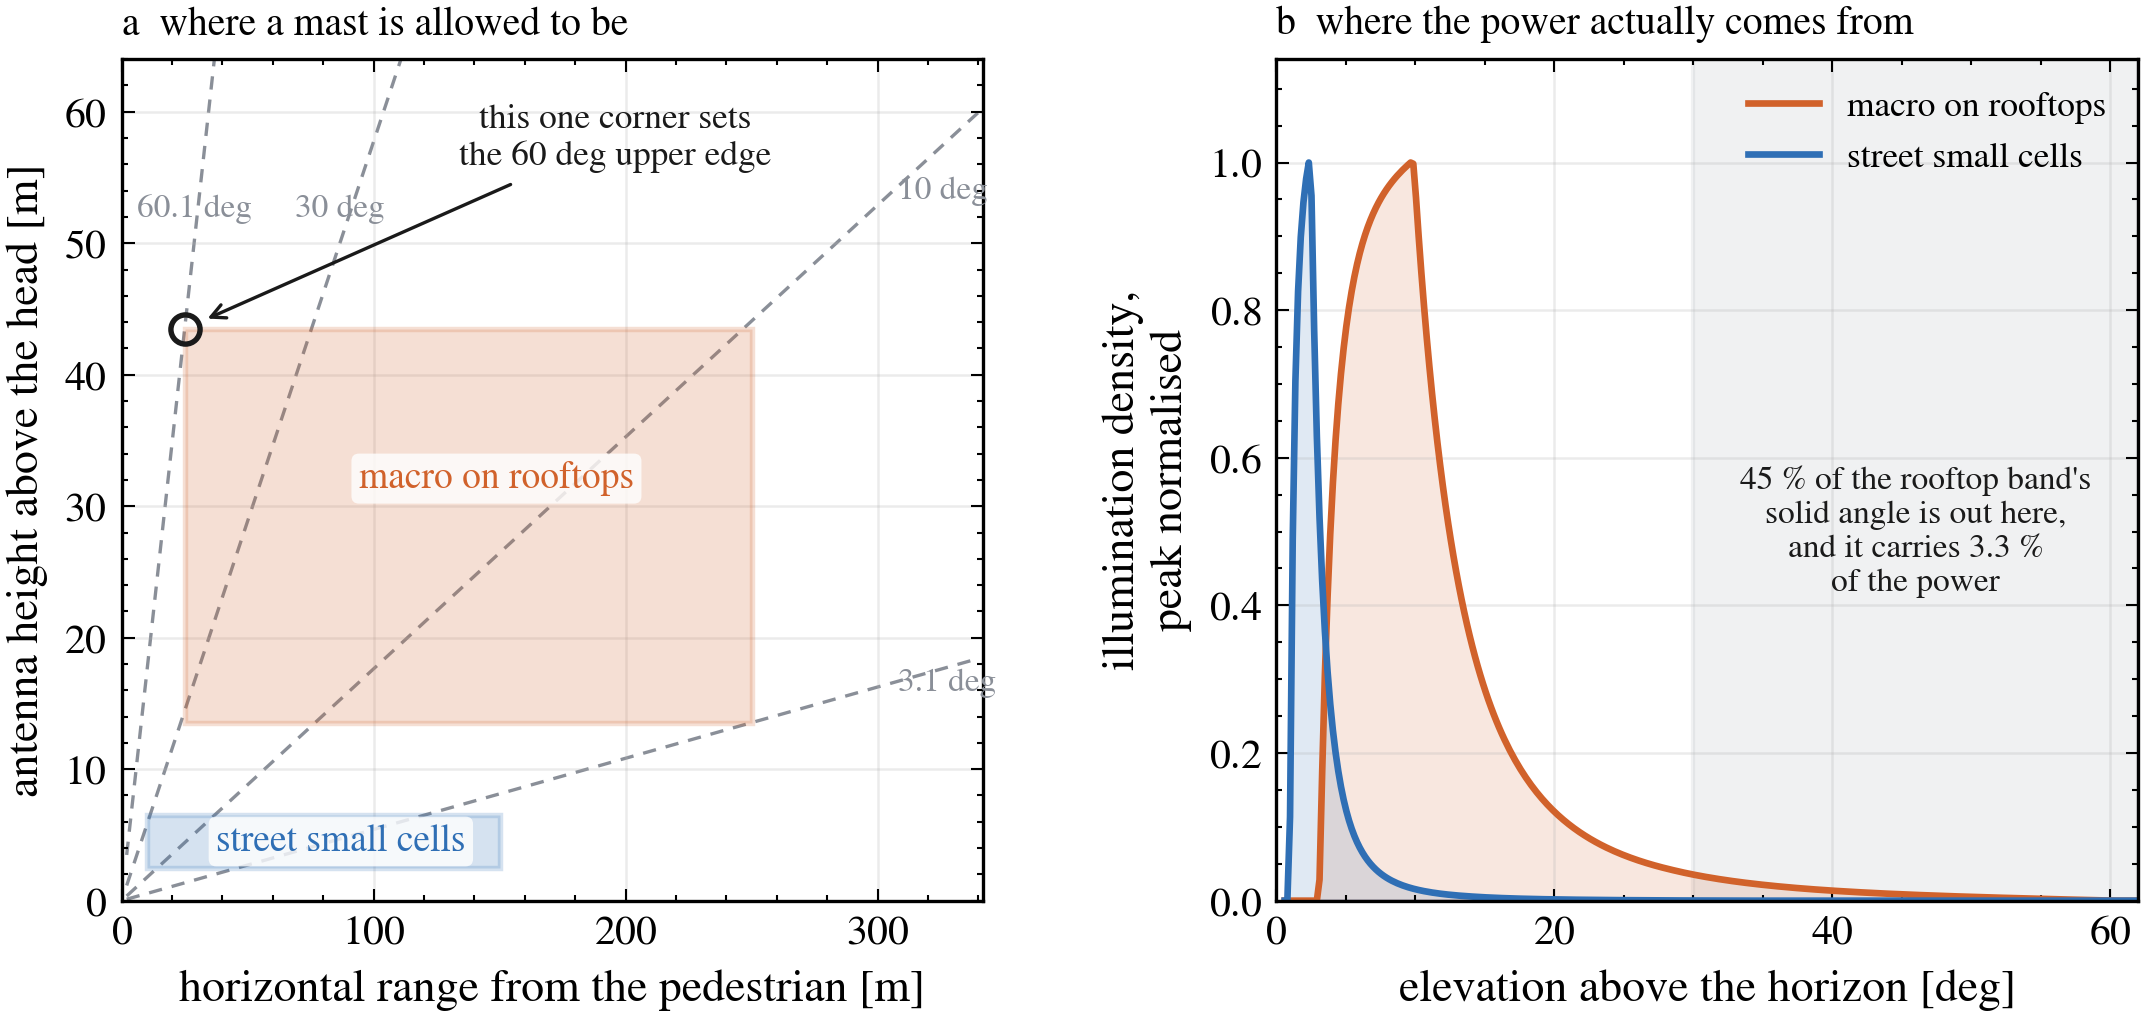
\includegraphics[width=\textwidth]{19_deployment_box}
  \caption{The region a site may occupy, in height above the head against
  horizontal range. Lines of constant elevation are straight through the origin,
  so the corners of the box set the elevation limits of \eqref{eq:support}.}
  \label{fig:box}
\end{figure*}

\subsection{Normalisation}

$Q$ is scaled so that it integrates to one over the sphere,
\begin{equation}
  \oint Q(\uext) \dOmega = 1 ,
\end{equation}
which is what makes $\chi$ dimensionless and equal to 1 in free space. The
integral is evaluated in elevation rather than on the ray grid, because
$Q$ concentrates within a few degrees of the horizon and a few hundred
grid cells cannot resolve that. The two elevations at which \eqref{eq:caps}
changes branch are inserted into the quadrature abscissae so that no interval
straddles a kink.

The normalisation hides the absolute level on purpose, which makes it easy to
forget to ask what $\chi$ multiplies. The same site density answers that. With
$\nu$ sites per unit volume of the slab, each radiating $P$, free space gives
\begin{equation}
  S_0 = \frac{P \nu}{4\pi} \oint \left( \rho_+ - \rho_- \right) \dOmega ,
  \label{eq:absolute}
\end{equation}
which is the cone integral of \eqref{eq:cone} again, now weighted by free space
spreading instead of counting sites. The $\rho_+ - \rho_-$ here is the same
object as the spreading variant of A4, used deliberately: an absolute level is a
question about how power adds, not about how a network shares it out. Over a
plausible range, 25 to 100 sites per
square kilometre radiating 55 to 75\,dBm, this puts $S_0$ between 0.0075 and
3.0\,W/m$^2$ for the rooftop band and between 0.010 and 4.1\,W/m$^2$ for the
street level band, against a general public reference level of 10\,W/m$^2$ at
this frequency \cite{icnirp}. Nearly three orders of magnitude, set entirely by
numbers that are not public. That spread is the reason this paper reports a
ratio: the part that depends on the square is measurable and transfers between
cities, and the part that depends on the network is neither.

\subsection{Models used}

Three illumination models are carried through every run. Their parameters are in
\cref{tab:models}. The isotropic model is a control rather than a deployment: it
weights all directions equally, so under it $\chi$ is exactly the fraction of
the sphere that is open sky, which makes it a check on the estimator as well as
a reference. The rooftop model covers macro sites on buildings and the street
model covers small cells on lamp posts and facades. Their height bands come from
the two ways operators acquire sites, a roof lease or a street furniture lease,
and published deployment heights are bimodal between them rather than spread
across the gap. Because no cellular deployment above 6\,GHz exists in the
European antenna registers, the band edges are not calibrated against measured
millimetre wave siting, and the sensitivity of $\chi$ to them is reported rather
than assumed.

\begin{table}[!t]
  \caption{Illumination models}
  \label{tab:models}
  \centering
  \begin{tabular}{lccc}
    \toprule
    Model & Height above head (m) & Range (m) & Elevation (deg) \\
    \midrule
    Isotropic & -- & -- & $-90$ to $90$ \\
    Rooftop macro & 13.5 to 43.5 & 25 to 250 & 3.09 to 60.11 \\
    Street cell & 2.5 to 6.5 & 10 to 150 & 0.95 to 33.02 \\
    \bottomrule
  \end{tabular}
\end{table}

\subsection{Beam pointing}

A base station at 15\,GHz is an array, not a point radiator, so a reader will
ask what beamforming does to all of this. It depends only on whether the beam
follows the person, and the case that sounds hardest is the one that changes
nothing at all.

Suppose every site puts its peak on the pedestrian. Under A1 each source is a
plane wave from one direction, so aiming at the pedestrian means peak gain along
$-\uext$ whatever the ray did on its way out of the square. The gain toward the
head is then the same constant for every site, so it multiplies \eqref{eq:Q} and
the normalisation divides it straight back out. $Q$ is not approximately
unchanged, it is the same function, and the estimator of
Section~\ref{sec:estimator} reads $Q$ only when depositing an escaped ray and
never inside a random draw, so the traced $\chi$ comes out bit identical.

For one policy this is exact and needs nothing else. Under full digital maximum
ratio transmission the site transmits along its own channel to the head, and a
matched filter delivers the total power in that channel whatever the channel is.
An array of $MN$ elements multiplies that total by $MN$ in the square and by the
same $MN$ over open ground, so the array factor cancels between numerator and
denominator with no assumption about how the paths are arranged.

The other matched policies only look invariant, and the difference matters
because they are the ones real networks use. A site that steers at the
pedestrian's coordinates aims at the direct path. A reflected path leaves that
site toward its own last surface, which can be a hundred metres from the head,
so it departs tens of degrees off the beam axis and the array puts it 20 to
25\,dB down. Geometric steering therefore suppresses the very multipath this
paper is measuring and pushes $\chi$ toward its no bounce value. Codebook beam
selection, which is what 5G beam management does, sits in between. Treating each
site as a single far point makes that offset vanish and both policies then read
as invariant, so the invariance there is an artefact of the far source picture
rather than a property of the physics. The direction of the error is at least
known: the numerator's gain is the peak times a sidelobe factor no greater than
one while the denominator's is the peak itself, so steered $\chi$ can only fall
below the value reported here.

One thing never cancels under any policy. The element pattern multiplies each
path before the aperture combines anything, so it survives as a reweighting of
$Q$. For a standard element that is a mild elevation taper, 0.26\,dB at the
rooftop model's median elevation of $9.5^\circ$ and 10.2\,dB at the
$60^\circ$ top of the band.

What does move $\chi$ is radiation that is not aimed at the person. A broadcast
beam carries a fixed electrical downtilt, and a beam serving another user points
somewhere else entirely. In both cases the gain becomes a function of elevation
and no longer factors out of the normalisation, so it reweights
\eqref{eq:Q} instead of cancelling. Since the elevation weighting is what
separates one square from another, a fixed pattern can reorder them, and that
variant is carried alongside the three models above.

\section{Adjoint ray estimator}

Reciprocity lets the trace run backwards. A ray leaving $\x$ in direction
$\uloc$, reflecting off surfaces and finally escaping in direction $\uext$ with
a surviving fraction $w$ of its launch power, describes the same physical path
as a wave arriving from a source at $\uext$ and reaching $\x$ from $\uloc$,
attenuated by the same $w$.

That reversal is what makes \eqref{eq:chidef} computable. A ray launched into
$\uloc$ and escaping into $\uext$ collects from the sources that lie in $\uext$,
which carry a share $Q(\uext)$ of the incident power, and it delivers a fraction
$w$ of it. Averaging over the rays launched into $\uloc$ gives the power arriving
from that direction, in units of $S_0$, and integrating over all launch
directions gives back the ratio itself,
\begin{equation}
  \Phi(\uloc) = \big\langle\, w \, Q(\uext) \,\big\rangle_{\uloc} , \qquad
  \chi = \oint \Phi(\uloc) \dOmega .
  \label{eq:chi}
\end{equation}
Nothing about the sources survives except $Q$, so one outward trace answers
\eqref{eq:chidef} for every source position at once. The free space denominator
$S_0$ never has to be computed, because $Q$ was normalised to make it 1.

\subsection{Estimator}
\label{sec:estimator}

The sphere of launch directions is divided into $M$ cells of near equal solid
angle using a Fibonacci grid. $N$ rays are launched in uniformly random
directions and each is assigned to the cell $c(j)$ nearest its launch direction,
giving $n_c$ rays in cell $c$. Escaping rays deposit into their launch cell, and
the estimate is the cell mean carried through the quadrature,
\begin{equation}
  \hat{\chi} = \frac{4\pi}{M} \sum_{c=1}^{M} \frac{1}{n_c}
  \sum_{j\,:\,c(j)=c} w_j \, Q(\uext_j) .
  \label{eq:estimator}
\end{equation}
Stratifying by launch cell rather than averaging over all rays at once matters
because $Q$ varies by orders of magnitude across the sphere, so an unstratified
average would be dominated by the few rays that happen to escape near the
horizon. In free space every ray escapes unobstructed with $w = 1$ and
$\uext_j = \uloc_j$, so \eqref{eq:estimator} reduces to a quadrature of $Q$ over
the sphere and returns 1, as it must.

Every ray either escapes without touching anything or reflects at least once, so
the sum in \eqref{eq:estimator} splits in two with nothing left over,
\begin{equation}
  \chi = \chi_{\mathrm{dir}} + \chi_{\mathrm{ref}} ,
  \label{eq:split}
\end{equation}
where the first term collects the untouched rays and the second collects the
rest. This separates the only two things a square can do. It hides part of the
sky, which removes direct power, and it reflects, which puts power back. The
first term is the direct arrival reduced by exactly the sky the buildings cover,
and under the isotropic model it equals the sky fraction, meaning the share of
directions from the head that reach open sky without meeting anything. That
equality is one of the identities checked in Section~\ref{sec:valid}. The second term is everything the
surroundings return. The split is a partition of the same rays, so it costs
nothing, and both parts are reported because a $\chi$ near 1 can mean an open
square or a closed one that reflects back what it blocked.

The estimator is stochastic, so every reported value carries a Monte Carlo
standard error, obtained by retracing the same standpoints over disjoint seed
streams rather than estimated from within a single run. Seeds and ray counts are
in the supplementary information.

How large that error is depends strongly on which illumination model is being
evaluated, and the reason is worth stating because it decides how many rays a
result needs. The variance is set by the share of the ray budget that lands
inside the support of $Q$. The isotropic model has support everywhere, so every
ray contributes and the per standpoint error is a few thousandths of a decibel.
The street model crowds its entire mass into the lowest tens of degrees of
elevation, so most rays escape into directions where $Q$ is zero and contribute
nothing, and the per standpoint error is some thirty times larger. Stratifying
the launch directions does not help with this, because the launch direction is
not the escape direction and only the latter is weighted. Reporting a median over
many standpoints does help, by roughly the square root of their number, which is
why a distribution over standpoints is the right unit for a claim and a single
standpoint often is not.

\subsection{Bounce loop}

\Cref{alg:trace} gives the loop and \cref{fig:oneray} follows a single ray
through it. Two steps deserve a word.

Roughness splits the reflection rather than blurring it. At each interaction the
fraction of reflected power that survives as a mirror reflection is the Rayleigh
factor
\begin{equation}
  \kappa = \exp\!\left[ -\left( \frac{4\pi \sigma_h \cos\theta_i}{\lambda}
  \right)^{\!2} \right] ,
  \label{eq:rayleigh}
\end{equation}
and the outgoing direction is drawn as a mirror reflection with probability
$\kappa$ and from a cosine weighted lobe about the normal otherwise
\cite{beckmann}. Choosing one lobe with a probability equal to its share of the
energy needs no compensating weight, because the two cancel. Note the
$\cos\theta_i$ in \eqref{eq:rayleigh}: a surface that scatters at normal
incidence behaves as a mirror at grazing incidence, and this is the only place
where that angle dependence enters.

Rays still travelling after $L$ interactions are dropped, and the power they
were carrying is reported as a share of the total, so the truncation is a
measured quantity rather than an assumption. Section~\ref{sec:budget} gives that
share and what follows from it.

\subsection{Bounce budget}
\label{sec:budget}

$L = 3$, and the reason is where the material evidence stops rather than where
the number stops moving. Two things have to be said straight away, because
without them this reads as a contradiction of
Section~\ref{sec:materials} and as a number chosen for cost.

The evidence in question is not a permittivity value.
Section~\ref{sec:materials} settled that those are interchangeable across
masonry. It is evidence of which family a surface belongs to, masonry against
glass or metal, which is the one material distinction that does move $\chi$ and
the one the mesh cannot supply on its own. So the budget is set by where
observed family membership stops, not by where a number stops being known to
three decimals.

The evidence leg is not unlimited either, and the measurements below say where
it runs out rather than leaving that to a reader to wonder about. A convergence
threshold would be the usual argument in place of all this, and it is not weaker
so much as insufficient by itself, since it shows the discarded tail is small
without showing the kept part is right. Both legs are used here, and the
convergence one comes last.

Two different questions hide inside the phrase ``observed surface'', and they
have to be separated or the numbers below look like they disagree. The first is
geometric: can the observation point see this surface at all? The second is
evidential: of the surfaces it can see, which did a camera actually photograph?
The first is a property of the formulation and holds in any square. The second
is a property of this particular set of panoramas.

Take the geometric question first. A photograph taken from the observation point
sees exactly the surfaces a ray can reach on its first interaction, so the first
hit is covered by construction. For a path that returns to where it started the
cover reaches the second interaction as well, since both ends of a closed loop
are seen from the same viewpoint. That is the co-located picture of
Section~\ref{sec:ratio} in its strictest form, and it is not a hypothetical.
Traced on the photogrammetric mesh at twelve standpoints, the share of returning
power whose whole chain lies on visible surfaces is 1.000000 at the first order
and 0.999991 at the second. It falls to 0.984 at the third, because the cover is
over the two ends of a loop and not over its middle.

An outward path gives up half of that, and this is what the adjoint move costs.
A ray leaving the first facade travels away from the viewpoint that saw it, so
only its first hit is assured. On the same geometry an outward path holds 0.999
at the first interaction, 0.916 at the second and 0.736 at the third, so by the
second interaction the estimator is already carrying 8\,\% of its power over
surfaces the standpoint cannot see, and by the third 26\,\%.

The evidential question is the stricter one, because a camera has to have stood
somewhere and looked. Where one did, the two questions coincide: the share of
incident power landing on a triangle some panorama photographed is 0.978 to
0.999 at the first interaction, across seven of the eight registered stations at
the reference square, which confirms the geometric argument to about two parts
in a thousand. The eighth returns 0.362, and since it stands eight metres from
one scoring 0.999 that is a registration failure rather than a coverage one. It
had passed the skyline residual gate, so first interaction coverage is the
sharper test of a pose, and that station is excluded. Away from a camera the two
questions come apart, and the reach turns out to be a radius. Within 20\,m of a
registered panorama the second interaction still lands on photographed material
93 to 96\,\% of the time and the third about 89\,\%, while beyond 40\,m every
depth falls below 0.21. Pooled over the published walk, which spans 90\,m, first
interaction coverage is 0.479. So the evidential claim is about a twenty metre
neighbourhood of the instrument rather than about a square, and every result
that uses image derived material carries that number beside it. These
percentages and the geometric ones above come from different standpoint sets at
different crop radii, so they answer the same question in different places and
are not to be differenced.

Three is then the smallest budget that lets both questions be asked. One
interaction would test nothing beyond the assured hit, two would show whether
the walk covers the square, and three shows what the first clearly unobserved
interaction is worth.

What makes three sufficient rather than merely defensible is where the power is.
Of all launched power, 10.7\,\% never touches a surface and escapes straight
to the sky, which is the direct term of \eqref{eq:split}. A further 79\,\%
interacts exactly once, 8.9\,\% twice, 1.2\,\% three times and 0.22\,\% ever
again. Depths past the third can be justified
neither by evidence nor by the power they carry. Traced against an eight
interaction reference over 40 of these standpoints at fixed seeds, so that only
the budget moves, $L = 3$ costs a median of 0.002\,dB and never moves a standpoint by more
than 0.12\,dB. Not one standpoint of the 40 moves half a decibel under any of
the three illumination models.

One consequence has to be stated plainly. A fixed budget is a hard cut, so the
estimator is truncated and therefore biased low, since truncation deletes power
and never adds it. The share of escaping power still in flight when the budget
runs out is 0.0038 at the median standpoint and 0.021 at the worst, and every
value reported here is a lower bound in that sense. That is not the same number
as the 0.22\,\% above, because the denominators differ: one is a share of all
launched power and the other a share of the power that actually escapes. Russian roulette is the
standard way to end paths without introducing this bias \cite{arvokirk}, but it
cannot repair a hard cap, and at a budget of three it would fire exactly once,
one step before the cap, killing rays at a 0.05 survival floor and inflating the
few survivors twentyfold. Measured over the same standpoints that is a worse
estimator at the same cost, so it is switched off. What the trace itself then
approximates reduces to a single one sided truncation whose size is quoted
above. The assumptions of Section~\ref{sec:ratio} sit underneath that and are
not part of the claim.

\begin{algorithm}[!t]
\caption{Adjoint trace at one standpoint}
\label{alg:trace}
\begin{algorithmic}[1]
\State $\hat{\Phi} \gets 0$
\For{$j = 1$ to $N$}
  \State draw $\uloc_j$ uniformly on the sphere, $c \gets$ nearest grid cell
  \State $w \gets 1$, $\uext \gets \uloc_j$
  \For{$b = 0$ to $L$}
    \State intersect the scene along $\uext$
    \If{no hit}
      \State $\hat{\Phi}[c] \gets \hat{\Phi}[c] + w\,Q(\uext)$
      \State \textbf{break}
    \EndIf
    \State $w \gets w \, |\Gamma(\theta_i, \varepsilon_r)|^2$
    \State with probability $\kappa$ set $\uext$ to the mirror direction,
    \Statex \hspace{\algorithmicindent} otherwise draw it cosine weighted about $\nhat$
  \EndFor
  \State \Comment{the loop ends at $b = L$ and whatever is still
  \Statex \hspace{\algorithmicindent} in flight is discarded}
\EndFor
\State \Return $\hat{\chi}$ from \eqref{eq:estimator}
\end{algorithmic}
\end{algorithm}

The cost is $O(N L \log T)$ for $T$ scene triangles, the logarithm coming from
the bounding volume hierarchy. Memory is $O(M)$ per standpoint, since no path is
stored: the trace keeps angular histograms and scalar sums only.

\begin{figure*}[!t]
  \centering
  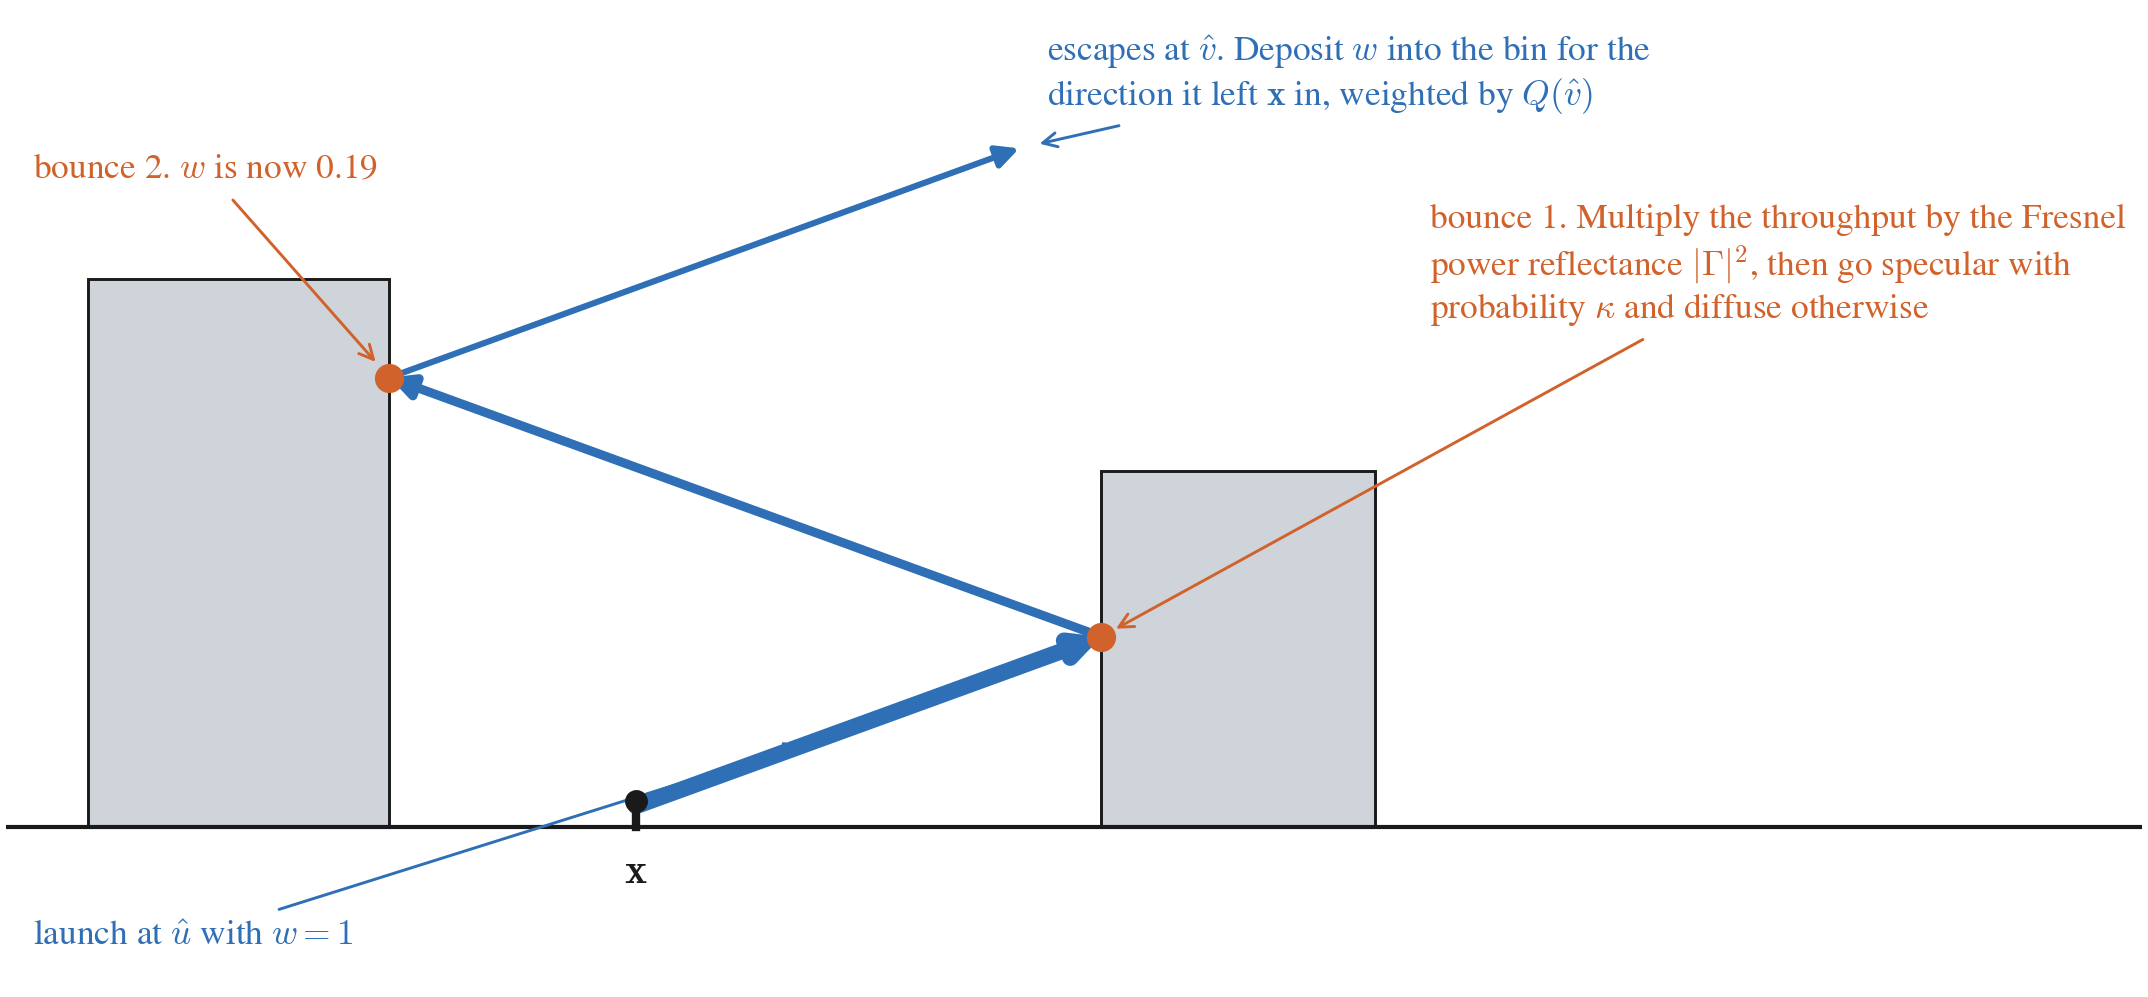
\includegraphics[width=\textwidth]{21_one_ray}
  \caption{One ray leaving the head, reflecting twice off facades and escaping
  to the sky. Line thickness is the surviving power $w$. The ray deposits
  $w\,Q(\uext)$ into the angular cell it was launched into, not the one it
  escaped through.}
  \label{fig:oneray}
\end{figure*}

\subsection{Quantities that come for free}

Two further quantities fall out of the same trace at no extra cost, on top of
the split in \eqref{eq:split}. The sky fraction, already met above, is reported
on its own because it depends on the geometry alone and on no illumination
model. The mean excess path length, taken over escaping rays weighted by their power, gives
the delay spread the square would impose. Both are reported alongside $\chi$.

\section{Body coupling}

The trace gives the power arriving at $\x$ from each direction. Turning that
into absorbed power on a body is a separate calculation and is done with an
established phantom and tissue model rather than reimplemented here
\cite{aegis, itis}. For a facet with outward normal $\nhat$ under a plane wave
travelling along $\khat$,
\begin{equation}
  S_{ab} = S_{\mathrm{inc}} \, T_0 \, \max\!\left[ \nhat \cdot (-\khat),\, 0
  \right] ,
  \label{eq:sab}
\end{equation}
where $T_0$ is the power transmitted into skin at normal incidence at 15\,GHz
and the clamp removes facets that face away. The arriving distribution
$\Phi(\uloc)$ is passed in as a set of plane waves, one per angular cell, with $\khat = -\uloc$, as reciprocity requires. Summing
\eqref{eq:sab} over cells gives the absorbed power density map on the body, and
integrating that map gives the absorbed power and the whole body specific
absorption rate.

Two things are left out of this step, and the first matters more than its size
suggests. The phantom stands alone. A bystander is not a small perturbation at
15\,GHz: a person is roughly thirty wavelengths across and optically thick, so
another body is opaque geometry rather than something a wave works around. What
makes a crowd different from a building is that it stands at the head's own
height. A standing adult reaches about 1.73\,m against an observation height of
1.5\,m, so a bystander adds only some 0.23\,m above the head, and a ray leaving
at elevation $\alpha$ clears the crowd after a horizontal distance
$0.23\,\mathrm{m} / \tan\alpha$. That is 13\,m at $1^\circ$, 2.6\,m at
$5^\circ$ and 0.4\,m at $30^\circ$. A crowd is therefore opaque along the
horizon and transparent above roughly $10^\circ$, and no crowd density changes
that.

The obvious next step is to predict each model's sensitivity from how much of
its measure sits near the horizon, and it is instructive that this fails. The
street level model sends 88\,\% of its measure below $5^\circ$ and the rooftop
model 9\,\%, a ratio of nine. The shares that actually arrive at the head are
0.21 and 0.19, a ratio of 1.15. The facades have already redistributed the power
before any crowd sees it, so a dense European square is its own near horizon
blocker and a crowd is a second edit to a distribution the buildings have
already set. Measured at twelve standpoints against paired empty square
baselines, two people per square metre cost a median 1.4\,dB under the street
model and 1.0\,dB under the rooftop model, and an ordinary busy 0.3 per square
metre costs 0.5 and 0.3\,dB. The isotropic control loses only 0.05\,dB, and
the reason is that weighting every direction equally makes redistribution free
and leaves only absorption to pay for. That is measured rather than argued:
repeating the run with the bodies replaced by index matched absorbers, so that
the geometry and the blockage are identical and only the reflected half is
removed, takes the isotropic loss from 0.05 to 0.71\,dB while the rooftop and
street columns move only from 1.04 to 1.33 and from 1.39 to 1.61\,dB. A crowd
is invisible to the isotropic control because it reflects, not because it fails
to block.

The second omission is that the body is treated as convex, so one limb never
shadows another, which matters most for arrivals that graze along it.

\section{Validation}
\label{sec:valid}

The estimator is checked in three ways, ordered from those that need no
reference value to those that need a reference calculation.

\subsection{Identities}

Some results follow from the construction and must come out exactly. Under the
isotropic model $\chi$ must equal the sky fraction, because weighting all
directions equally means the answer is the open solid angle and nothing else,
and the two are computed by different code paths. In an empty scene every model
must return $\chi = 1$. Reversing every path must leave the transported power
unchanged. Total reflected power must never exceed incident power at any
interaction. These are property tests over randomised inputs rather than single
cases.

\subsection{Closed forms}

Two geometries have analytic answers. A single infinite ground plane below the
standpoint gives a $\chi$ that can be written down from \eqref{eq:cone} and the
Fresnel coefficient alone. A Lambertian spherical cavity gives a second, with a
different balance between the direct and the multiply reflected contribution.
Both are reproduced to the tolerance set by the ray count.

\subsection{Convergence}

Two parameters are measured here, and a third is corroborated rather than
chosen. The bounce budget $L$ is fixed by evidence in
Section~\ref{sec:budget}, and the trace out to eight interactions reported
there is what corroborates it. That comparison needs one remark, because the obvious way to read it is
wrong. Two runs that differ only in $L$ and share a seed trace the same rays and
agree exactly up to the shallower depth, so their difference is paired and is
resolved far better than either value is on its own. Reading it against the single run
error of Section~\ref{sec:estimator} would make a real and well measured
difference look like noise. The ray count $N$ is raised until the spread across
independent seeds falls below the differences being interpreted. The crop radius is raised until
$\chi$ stops moving, which is what fixes the 250\,m figure quoted in
Section~\ref{sec:config}: at smaller radii the mesh is missing buildings that
would have
blocked near horizon paths, and the near horizon is where the illumination
models put most of their measure. The converged radius is a property of the
illumination model and not of the square, so it is reported per model.

One radius converges and one does not, and they are easy to confuse. The crop
radius above is the extent of the mesh. The outer radius $\rho_+$ of the
deployment box in Section~\ref{sec:illum} is a different number, and sweeping it
from 50 to 500\,m never reaches a plateau: $\chi$ falls about as
$\rho_+^{-1.2}$, worth 7.4\,dB at the median square for the rooftop model. That
is not a defect of the estimator, it is what a uniform site density over an
unbounded plane does, since the lower edge of the elevation support keeps
sliding toward the horizon. It means no absolute $\chi$ can be quoted without
the radius it was computed at. What is far steadier is the contrast between
squares, which moves 0.51\,dB against that 7.4\,dB, and that is the quantity the
results lead with. The sweep costs no extra tracing, for the same reason the
adjoint move works: $\chi$ is linear in the illumination density and every band
law is uniform in azimuth, so one trace collapses to an elevation histogram and
any choice of box is a dot product against it. Every radius is therefore scored
on identical rays.

Identities and closed forms constrain the implementation, not the formulation.
A derivation error that is coded faithfully passes all of them, and one such
error was in fact found by rederiving \eqref{eq:cone} rather than by any test
failing. What guards against that class of error is a second calculation that
shares no code with the first. The diffraction bound of A6 provides one as a
by-product: its mask, its quadrature and its ray budget are independent of the
estimator, and integrating it over the visible directions instead of the
shadowed ones reproduces the estimator's own direct term to within 0.34\,\%
isotropic, 1.73\,\% rooftop and 7.3\,\% street. Only the direct term is covered
by it. The reflected term has no independent check at the time of writing.


\section{Results}
\label{sec:results}

The results use the geometric material assignment at every square, a 250\,m
crop, three surface interactions, and the corrected illumination law. Each of
the eleven squares contributes 80 standpoints, giving 880 records with no torn
rows. \Cref{fig:city-scenes} shows the geometry set. The exposure run uses the
converged crop even where the overview image shows a smaller visual crop.

\begin{figure*}[!t]
  \centering
  \includegraphics[width=\textwidth]{11_eleven_cities}
  \caption{The configuration comprises eleven accepted photogrammetric city
  squares. Each panel uses framing derived from its own geometry. The rejected
  Istanbul mesh is retained in the overview to show the coarse source geometry
  that failed the admission criterion. Exposure is evaluated on the accepted
  squares with the common 250\,m crop.}
  \label{fig:city-scenes}
\end{figure*}

\subsection{Eleven squares}

The square changes the exposure ratio by several decibels. The between-square
spread is 3.71\,dB under isotropic illumination, 4.93\,dB under the rooftop
model, and 9.58\,dB under the street-cell model. Mexico City's Zocalo has the
largest exposure ratio. The largest spread inside one square is 6.46\,dB under
isotropic illumination in Madrid. It exceeds the spread between all eleven
square medians by 2.75\,dB. A single standpoint is therefore not a sufficient
description of a square.

\Cref{fig:eleven-exposure} gives the distributions for the corrected rooftop
law, the sky fraction, and the corresponding body-side peak absorbed power
density. The same geometric material prior is used everywhere. The fixed ground
datum removes the roof placements that had made Krakow and Toulouse outliers in
an earlier run. The correction changes Krakow by $-1.40$\,dB and Toulouse by
$-1.29$\,dB under isotropic illumination. Every other square changes by less
than 0.25\,dB under that model.

\begin{figure*}[!t]
  \centering
  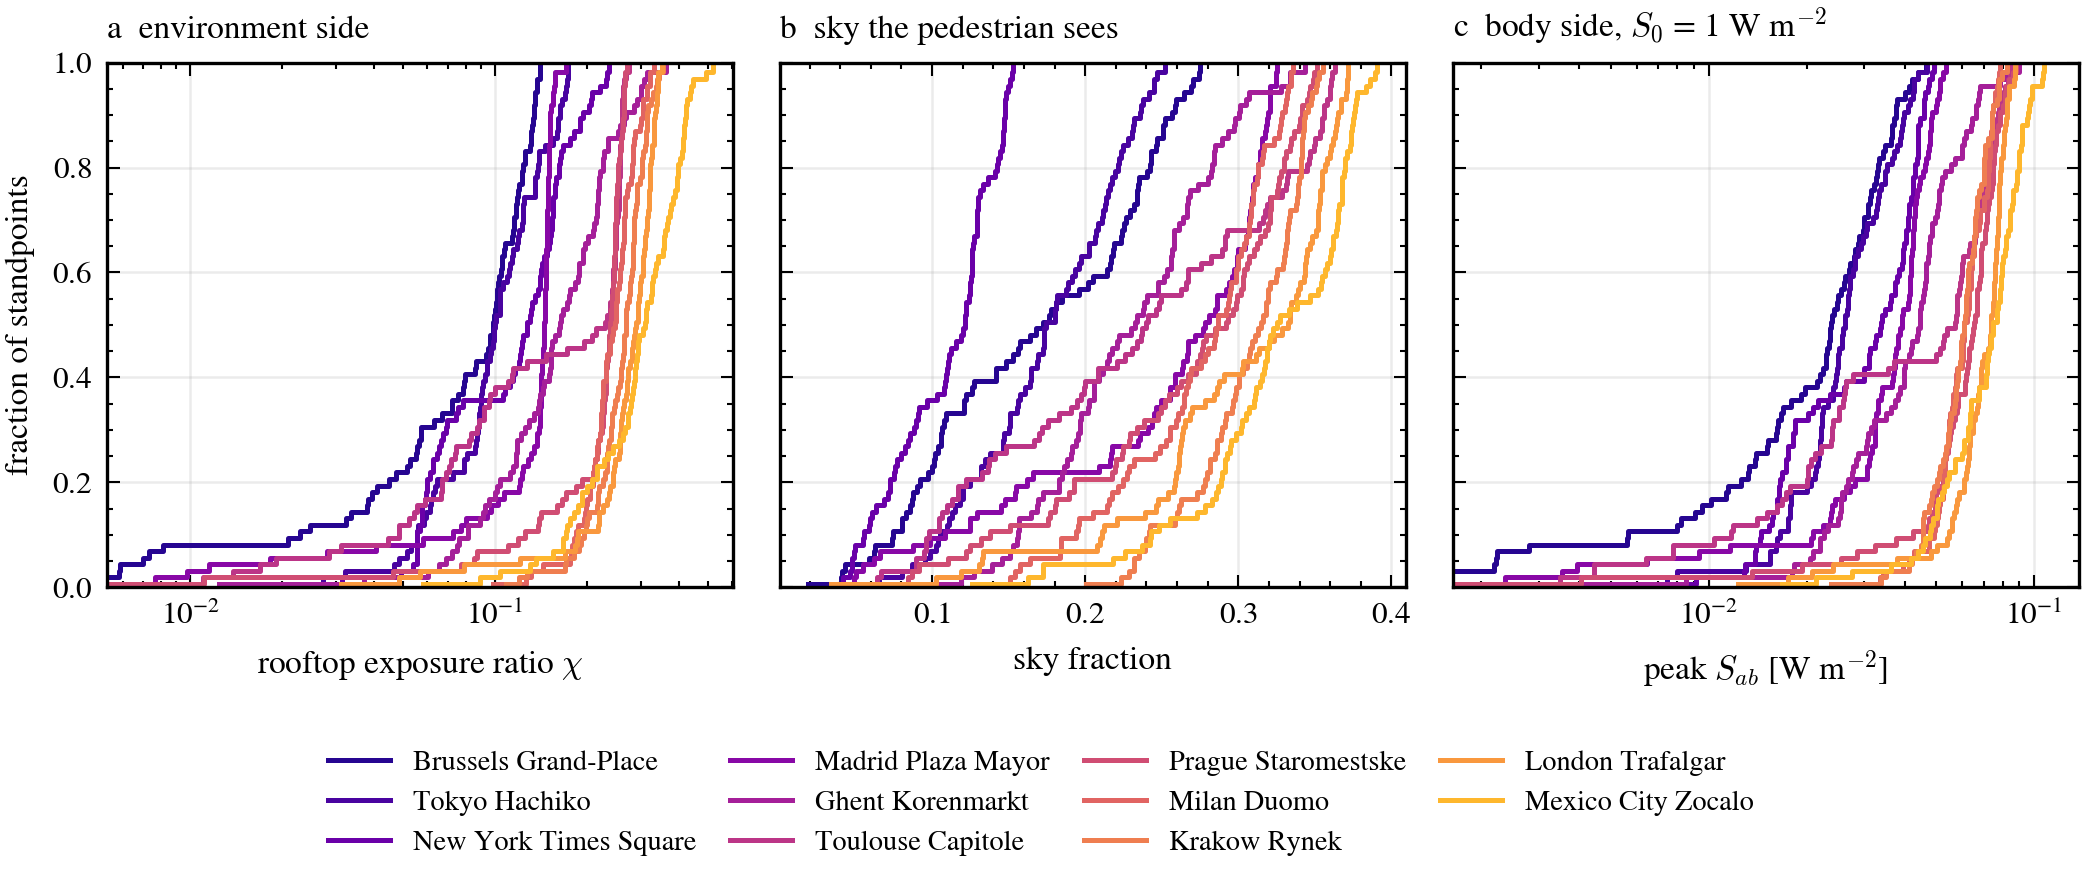
\includegraphics[width=\textwidth]{16_eleven_cities_exposure}
  \caption{The eleven-square distributions after convergence and the ground
  datum correction. The left panel gives the rooftop exposure ratio, the middle
  panel gives the sky fraction, and the right panel gives peak absorbed power
  density for an open-ground density of 1\,W/m$^2$. Each curve contains 80
  standpoints.}
  \label{fig:eleven-exposure}
\end{figure*}

\begin{table}[!t]
  \caption{Spread, material shift, and sampling error}
  \label{tab:result-summary}
  \centering
  \begin{tabular}{lccc}
    \toprule
    Illumination & Square spread & Material shift & Median s.e. \\
     & (dB) & (dB) & (dB) \\
    \midrule
    Isotropic & 3.71 & 0.024 & 0.0042 \\
    Rooftop & 4.93 & 0.029 & 0.0136 \\
    Street cell & 9.58 & 0.022 & 0.0343 \\
    \bottomrule
  \end{tabular}
\end{table}

\subsection{Illumination changes the order}

The illumination law changes which square appears most open to the network.
The rooftop ranking remains close to the isotropic ranking, with Spearman
correlation $+0.936$. The street-cell ranking has correlation $+0.345$ with the
isotropic order. Buildings intercept the near-horizon support of the street
model much more strongly than the higher rooftop support. The corrected site
count law therefore reorders the squares instead of applying one common offset.
This is the largest modeling choice in the comparison because the reported
ratio belongs jointly to a square and an illumination law.

\subsection{Material discrimination bounds the claim}

Two image-based material compositions that assign visibly different facade
classes give the same exposure distribution. Replacing the entity-based facade
prior with the image-derived material classes changes the distribution median by
0.024\,dB under isotropic illumination, 0.029\,dB under rooftop illumination,
and 0.022\,dB under street-cell illumination. \Cref{tab:result-summary} places
these shifts beside between-square spreads of 3.71, 4.93, and 9.58\,dB. Each
material shift remains below the scale needed to change a city ordering.

The null result licenses the geometric assignment only within the observed
material family. The photographs show that the reference square is masonry.
They do not estimate a finely tuned permittivity. A square dominated by glass
or metal remains outside the tested family because the mesh alone does not
identify that change. Material discrimination therefore sets the boundary of
the cross-city claim: the reported comparison applies to masonry squares.

\subsection{Beamforming depends on what the beam follows}

Full digital maximum ratio transmission cancels from the ratio exactly. The
matched filter collects the total channel power, and the array gain multiplies
both the real-square numerator and the open-ground denominator. The result needs
no assumption about how many paths reach the pedestrian or which directions
they occupy. The element pattern remains and changes the weighting by 0.26\,dB
at the rooftop median elevation of $9.5^\circ$ and by 10.2\,dB at the
$60^\circ$ top of the band.

Geometric steering and codebook selection do not share the exact cancellation.
A reflected path leaves the site toward its final surface, whereas a coordinate
steering beam points toward the head. The array can therefore suppress the
reflected numerator while retaining the direct open-ground denominator. The
result is one-sided: the steered ratio cannot exceed the value reported here.
The far-source approximation makes both directions coincide and hides this
difference. \todo{Run the geometric-steering and codebook-beam sweep to measure
the gap below the reported upper bound.}

\subsection{Bystanders alter the arriving distribution}

Geometry predicts strong elevation selectivity for a crowd. A standing adult
adds 0.23\,m above the head. A ray clears that height after 13\,m at
$1^\circ$, 2.6\,m at $5^\circ$, and 0.4\,m at $30^\circ$. Since the street and
rooftop models send 88\% and 9\% of their measure below $5^\circ$, the geometric
prediction was a factor of nine between their crowd losses.

The trace rejects that prediction. At two people per square metre, the street
model loses 1.4\,dB and the rooftop model loses 1.0\,dB. The ratio of losses is
1.4 instead of nine. The sent angular measure is not the arriving measure. The
arriving shares below $5^\circ$ are 0.21 and 0.19, a ratio of 1.15, because the
facades redistribute the power before it reaches the crowd. The isotropic model
loses only 0.05\,dB because equal weighting recovers power that bodies reflect
into another direction. The crop-radius measurement that follows is shown in
\Cref{fig:crop-convergence}.

\subsection{Crop radius is measured}

The crop radius follows from a convergence trace rather than a visual choice.
\Cref{fig:crop-convergence} holds the observers fixed and changes only the
surrounding geometry. Small crops omit distant buildings that block low-elevation
directions, so the directional models move first. Raising the radius until the
next larger crop no longer changes the interpreted ratio fixes the common
250\,m operating point. The convergence is measured separately for each
illumination law because each law weights the missing directions differently.

\begin{figure}[!t]
  \centering
  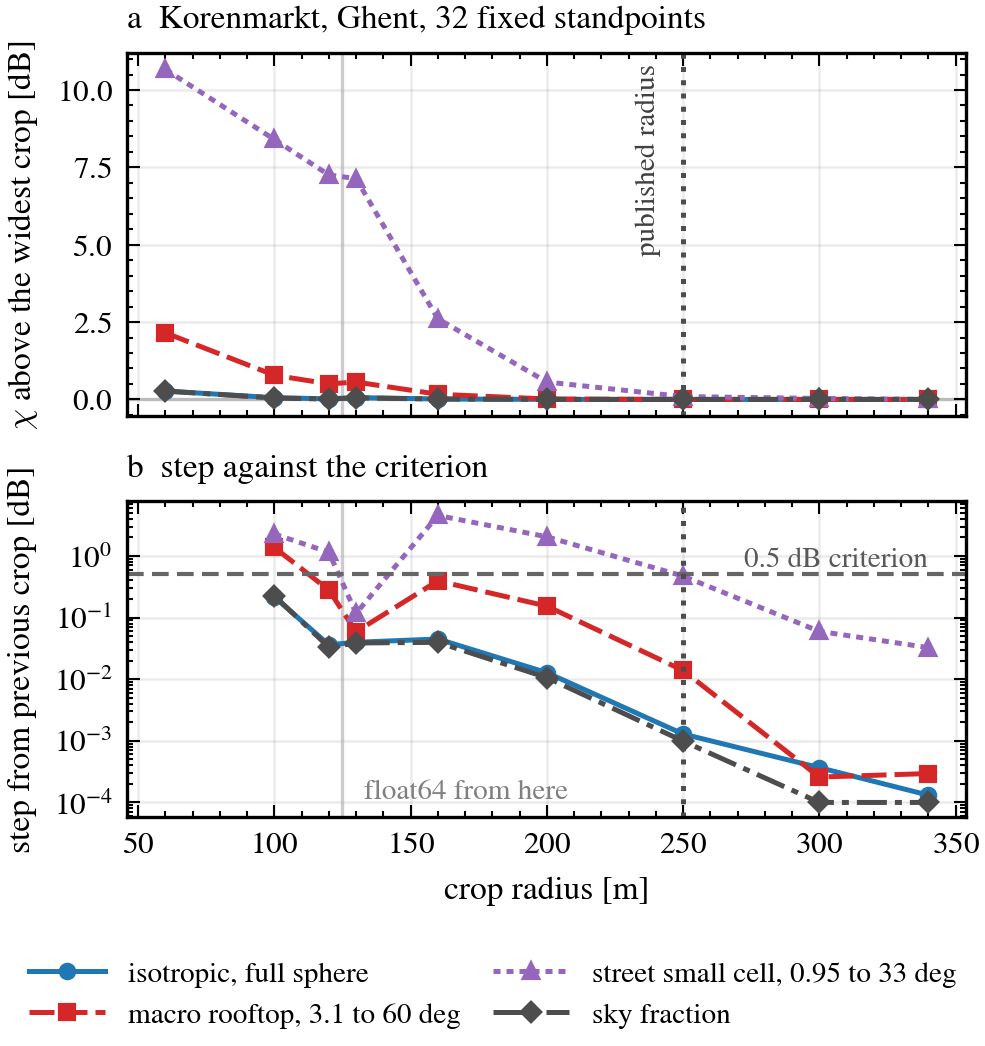
\includegraphics[width=\columnwidth]{15_crop_convergence}
  \caption{The crop-radius convergence measurement at fixed observers. The top
  panel gives each value relative to the widest crop. The bottom panel gives the
  change from the preceding radius. The illumination model determines how fast
  omitted low-elevation blockers cease to change the ratio.}
  \label{fig:crop-convergence}
\end{figure}

\section{Discussion and threats to validity}
\label{sec:discussion}

The results separate two sources of variability that an absolute exposure level
mixes together. The network sets the open-ground level. The square and the
illumination law set the ratio. A change in the illumination law can reorder the
cities, so the ratio is not a universal score attached to a mesh. It is a
response of that mesh to a stated source distribution. This qualification is
also its use: another deployment hypothesis can be applied without rebuilding
the square or choosing discrete transmitters.

The computation at the person is more than an amortization. At a camera
position, the first interaction is on a photographed surface by construction.
The second interaction retains 93\% to 96\% image coverage within 20\,m of a
registered panorama, and every depth falls below 0.21 beyond 40\,m. Across the
published 90\,m walk, first-interaction coverage is 0.479. The evidence is
therefore local to the instrument. Three interactions remain sufficient because
79\% of launched power ends after one interaction, 8.9\% after two, 1.2\%
after three, and only 0.22\% reaches a fourth interaction. Against an
eight-interaction reference, the three-interaction budget changes the median by
0.002\,dB and no standpoint by more than 0.12\,dB.

A co-located return does not replace the outward estimator. Across 440
standpoints, 98.6\% of the return is first order and its power-weighted two-way
range is 4.05\,m. Its median is $-70.81$\,dB against $-70.99$\,dB for a rough
half-space calculation. The instrument mostly sees its own pavement. The pooled
Spearman correlation with the exposure ratio is $-0.526$, but the partial
correlation at fixed sky fraction is $-0.010$. Sky fraction alone correlates at
$+0.961$. The second-order return retains a partial correlation of $-0.345$
with the reflected ratio, but it is 0.37\% of received power and sits 24\,dB
below the pavement return. The closed-loop geometry gives the image-visibility
guarantee. Its return amplitude is not a practical proxy for the exposure ratio.

The material result is a bound on generalization. Masonry substitutions move
the median by hundredths of a decibel because their reflection responses partly
cancel over many directions and standpoints. The experiment did not test a
glass-curtain-wall square or a metal-clad square. Applying the geometric facade
default there would change material family rather than refine a masonry value.
The null therefore supports the eleven-square comparison only because the
observed squares belong to the tested family.

\Cref{tab:honesty} states every known bias with its size and direction. Several
errors point low. Diffraction adds paths, facade polarization averaging loses up
to 3.0\,dB, and truncation deletes power. The ground-polarization error points
high near $24^\circ$ elevation and can reach tens of decibels on the affected
paths. The body self-shadow error and the diffuse-scattering error have unknown
signs. The latter is the larger physical risk. Published ablations move
prediction error from 6--13\,dB to 25--37\,dB at 28 and 38\,GHz when diffuse
scattering is removed~\cite{vitucci}.

\begin{table}[!t]
  \caption{Known biases, sizes, and directions}
  \label{tab:honesty}
  \centering
  \scriptsize
  \setlength{\tabcolsep}{2pt}
  \begin{tabular}{@{}p{0.24\columnwidth}p{0.51\columnwidth}p{0.17\columnwidth}@{}}
    \toprule
    Source & Measured or bounded size & Effect on $\chi$ \\
    \midrule
    Diffraction omitted & Median uplift 0.06, 0.15, and 0.44\,dB for isotropic,
    rooftop, and street illumination & Biases low \\
    Unpolarized facade average & At most 3.0\,dB & Biases low \\
    Unpolarized ground average near $24^\circ$ & Up to tens of decibels over
    7.8\% of rooftop measure and 0.4\% of street measure & Biases high \\
    Three-interaction truncation & 0.0038 of escaping power at the median &
    Biases low \\
    Convex body without limb self-shadow & Unquantified & Unknown \\
    Image evidence & One square on the material axis, with 0.479 pooled
    first-interaction coverage & Limits scope \\
    Failed registered station & Excluded at 0.362 first-interaction coverage &
    Limits scope \\
    Modeled diffuse split & Published error changes from 6--13\,dB to
    25--37\,dB when diffuse scattering is ablated at 28 and 38\,GHz & Unknown \\
    \bottomrule
  \end{tabular}
\end{table}

The sampling errors are smaller than the reported city spreads. The standard
errors of a walk median are 0.0042\,dB isotropic, 0.0136\,dB rooftop, and
0.0343\,dB street. One older street-cell evidence-ladder shift of 0.079\,dB is
only 2.3 standard errors and is not resolved. The earlier 0.298\,dB headline
used a superseded illumination law and has not been measured under the corrected
law. Neither value is used as a result here.

The bystander experiment adds a separate scope limit. It uses one masonry square
at one carrier with static upright people. Its mechanism is still informative:
the facades have already changed the arriving elevation distribution before a
crowd blocks it. Repeating the experiment in squares with different openness and
with measured pedestrian motion is required before treating the 1.4 and
1.0\,dB shifts as city-independent corrections.

\section{Conclusion}
\label{sec:conclusion}

This study showed that the shape of a city square changes relative pedestrian
exposure at 15\,GHz by several decibels after the unknown network level is
divided out. The illumination law changed the city order, so the result belongs
to the pair formed by the square and the assumed site distribution. Variation
inside one square exceeded the isotropic variation between eleven square
medians. A city value therefore needs a distribution of pedestrian standpoints.

Computing at the pedestrian joined propagation to observable evidence. A
co-located photograph covered the surfaces that received the early interactions,
and the measured decay of that coverage set the bounce budget. Material
discrimination inside the observed masonry family then changed the exposure
ratio by only hundredths of a decibel. The result establishes the boundary of
the claim: geometry carries the comparison among masonry squares, and image
evidence is needed to determine whether a new square belongs to that family.

Future work must first measure the gap between geometric steering, codebook
selection, and the reported beamforming upper bound. It must then fit diffuse
scattering and repeat the bystander study beyond one square, since those are the
largest unresolved physical and scope limits identified here.

\begin{thebibliography}{99}

\bibitem{icnirp}
International Commission on Non-Ionizing Radiation Protection, ``Guidelines for
limiting exposure to electromagnetic fields (100 kHz to 300 GHz),'' \emph{Health
Phys.}, vol. 118, no. 5, pp. 483--524, 2020.

\bibitem{leeman}
S.~Leeman, R.~Wydaeghe, S.~van~der~Straeten, Y.~Goegebeur, G.~Vermeeren, and
W.~Joseph, ``City-scale spatio-temporal modeling of 5G downlink exposure of
users and non-users by ray-tracing in a real urban environment,'' \emph{IEEE
Access}, vol. 13, pp. 30894--30906, 2025.

\bibitem{wydaeghe2026}
R.~Wydaeghe, S.~Shikhantsov, G.~Vermeeren, L.~Martens, E.~Tanghe, and W.~Joseph,
``Hybrid ray-tracing-QuaDRiGa/FDTD method for realistic 28 GHz exposure with 6G
CF-MaMIMO in 3D outdoor environments,'' \emph{npj Wireless Technol.}, vol. 2,
no. 1, Art. no. 13, 2026.

\bibitem{sionna}
J.~Hoydis, F.~A\"it~Aoudia, S.~Cammerer, M.~Nimier-David, N.~Binder,
G.~Marcus, and A.~Keller, ``Sionna RT: Differentiable ray tracing for radio
propagation modeling,'' in \emph{Proc. IEEE Globecom Workshops}, 2023,
pp. 317--321.

\bibitem{wiame}
C.~Wiame, S.~Demey, L.~Vandendorpe, P.~De~Doncker, and C.~Oestges, ``Joint data
rate and EMF exposure analysis in Manhattan environments: Stochastic geometry
and ray tracing approaches,'' \emph{IEEE Trans. Veh. Technol.}, vol. 73, no. 1,
pp. 894--908, 2024.

\bibitem{varsier}
N.~Varsier, D.~Plets, Y.~Corre, G.~Vermeeren, W.~Joseph, S.~Aerts, L.~Martens,
and J.~Wiart, ``A novel method to assess human population exposure induced by a
wireless cellular network,'' \emph{Bioelectromagnetics}, vol. 36, no. 6,
pp. 451--463, 2015.

\bibitem{veludo}
A.~F.~Veludo \emph{et al.}, ``Assessing radiofrequency electromagnetic field
exposure in multiple microenvironments across ten European countries with a
focus on 5G,'' \emph{Environ. Int.}, vol. 200, Art. no. 109540, 2025.

\bibitem{mmsv}
A.~Kamari, Y.~Chae, and P.~Pathak, ``mmSV: mmWave vehicular networking using
Street View imagery in urban environments,'' in \emph{Proc. 29th Annu. Int.
Conf. Mobile Comput. Netw.}, 2023, pp. 1--16.

\bibitem{veach}
E.~Veach, \emph{Robust Monte Carlo Methods for Light Transport Simulation}.
Stanford, CA, USA: Stanford Univ., Ph.D. dissertation, 1997.

\bibitem{tregenza}
P.~R.~Tregenza and I.~M.~Waters, ``Daylight coefficients,'' \emph{Lighting Res.
Technol.}, vol. 15, no. 2, pp. 65--71, 1983.

\bibitem{sloan}
P.-P.~Sloan, J.~Kautz, and J.~Snyder, ``Precomputed radiance transfer for
real-time rendering in dynamic, low-frequency lighting environments,'' in
\emph{Proc. 29th Annu. Conf. Comput. Graph. Interactive Techn.}, 2002,
pp. 527--536.

\bibitem{itu2040}
International Telecommunication Union, ``Effects of building materials and
structures on radiowave propagation above about 100 MHz,'' Recommendation
ITU-R P.2040-4, 2023.

\bibitem{sam}
A.~Kirillov \emph{et al.}, ``Segment anything,'' in \emph{Proc. IEEE/CVF Int.
Conf. Comput. Vis.}, 2023, pp. 4015--4026.

\bibitem{ericsson}
Ericsson, ``Street microcell channel measurements at 2.44, 14.8 and 58.68 GHz,''
3GPP TSG-RAN WG1 \#84, doc. R1-160846, Malta, Feb. 2016.

\bibitem{mmmagic}
mmMAGIC, ``Measurement results and final mmMAGIC channel models,'' Deliverable
H2020-ICT-671650-mmMAGIC/D2.2, 2017.

\bibitem{adhikari}
S.~Adhikari \emph{et al.}, ``Over-the-top propagation in urban millimetre wave
networks,'' in \emph{Proc. IEEE INFOCOM}, 2025.

\bibitem{p526}
International Telecommunication Union, ``Propagation by diffraction,''
Recommendation ITU-R P.526-16, 2024.

\bibitem{duchizhik}
J.~Du, D.~Chizhik, R.~A.~Valenzuela \emph{et al.}, ``Suburban and urban ducting
and around-the-corner propagation at 28 GHz,'' \emph{IEEE Trans. Antennas
Propag.}, vol. 69, no. 6, pp. 3459--3469, 2021.

\bibitem{vitucci}
E.~M.~Vitucci, V.~Degli-Esposti, F.~Fuschini \emph{et al.}, ``Ray tracing RF
field prediction: an unforgiving validation,'' \emph{Radio Sci.}, vol. 54,
no. 11, pp. 1112--1128, 2019.

\bibitem{karttunen}
A.~Karttunen, J.~J\"arvel\"ainen, S.~L.~H.~Nguyen, and K.~Haneda, ``Modeling the
multipath cross-polarization ratio for 5--80 GHz radio links,'' \emph{IEEE Trans.
Wireless Commun.}, vol. 18, no. 10, pp. 4768--4778, 2019.

\bibitem{beckmann}
P.~Beckmann and A.~Spizzichino, \emph{The Scattering of Electromagnetic Waves
from Rough Surfaces}. Oxford, U.K.: Pergamon, 1963.

\bibitem{arvokirk}
J.~Arvo and D.~Kirk, ``Particle transport and image synthesis,'' in
\emph{Proc. SIGGRAPH}, 1990, pp. 63--66.

\bibitem{aegis}
R.~Wydaeghe, ``AEGIS: absorbed power density on human bodies in wireless
environments,'' software, 2026.

\bibitem{itis}
P.~A.~Hasgall \emph{et al.}, ``IT'IS database for thermal and electromagnetic
parameters of biological tissues,'' Version 4.2, 2024.

\end{thebibliography}

\end{document}
